%************************************************
\chapter{L'elasticità della gomma}\label{chp:ElasticitaGomma}
%************************************************
\section{Cos'è l'elasticità?}
Ipotizzando un materiale cristallino, se posto ad una trazione: si sta cedendo energia al sistema.
Il quale equilibra la forza con una resistente che tende a riportare il sistema in una condizione di equilibrio a minore energia.

\begin{figure}
\centering
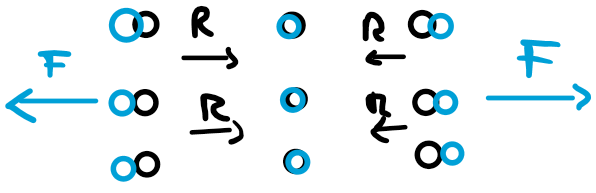
\includegraphics[width = 0.5\textwidth]{gfx/Elasticita}
\caption{Resistente per mantenere il materiale insieme}
\label{fig:Elasticita}
\end{figure}

La forza resistente è una forza elastica: dunque ci si aspetta che togliendo la forza di azione, la reazione riporti il materiale allo stato iniziale.

Prendiamo per esempio il caso di un pistone.
Se si applica l' ipotesi di quasi-statico: cioè la componente è talmente lenta da considerare la temperatura costante.

\begin{figure}
\centering
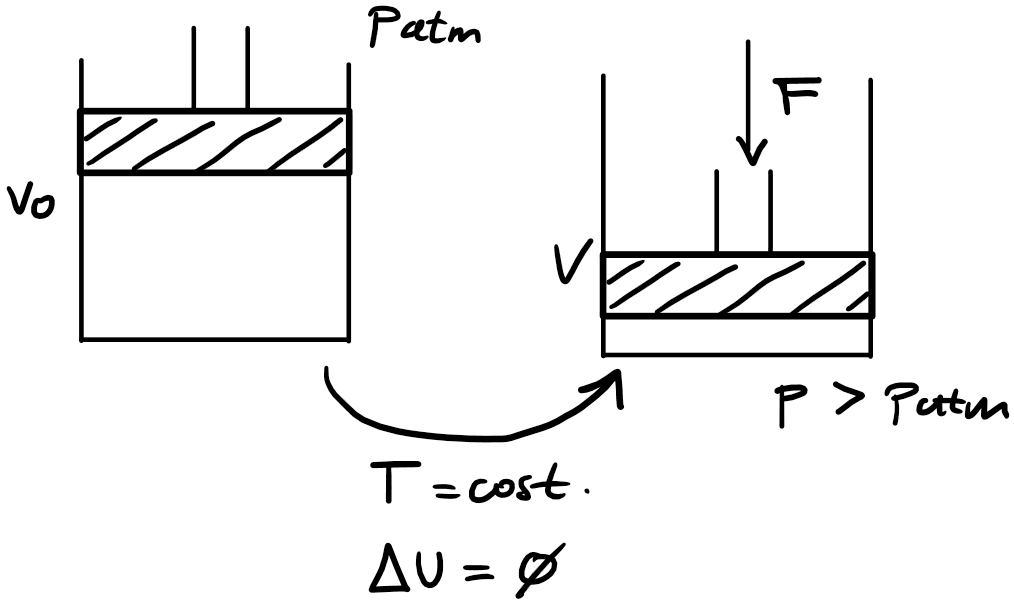
\includegraphics[width = \textwidth]{gfx/1Termodinamica}
\caption{Esempio del pistone per il primo principio della termodinamica}
\label{fig:1Termodinamica}
\end{figure}

Applichiamo il primo principio della termodinamica.

\paragraph{Primo principio della termodinamica}
\begin{equation}
dU = dQ - pdV
\end{equation}
Da cui seguendo le ipotesi di:
\begin{equation}
Hyp:%
\begin{cases}
T &= cost.\\
dQ &= TdS
\end{cases}
\end{equation}
Da cui:
\begin{equation}
0 = TdS - pdV \Rightarrow p = T\frac{\partial S}{\partial V}\Big|_{T = cost.}
\end{equation}
Interrogando l'equazione di Boltzman:
\begin{equation}
S = S_0 + K_b \ln(W)
\end{equation}
Dove $W$ è il numero di configurazione che il sistema può assumere, ovvero l'\textbf{entropia configurazionale}.
In generale si osserva che per una singola molecola $W \propto V$ mentre per $N$ molecole: $W \propto V^N$.
In particolare, la seconda conseguenza è dovuta al fatto che se una molecola ha un configurazione, le altre ne abbiano una completamente differente.
ne segue:
\begin{equation}
\begin{split}
S &= S_0 + K_b\ln(CV^N) = S_0 + K_b\left[\ln(C) + \ln(V^N)\right] =\\
&= S_0 + K_b N\left[\ln(C) + \ln(V)\right]=\\
&= S_0 + K_b N \ln(V)
\end{split}
\end{equation}
Applicando al primo principio della termodinamica:
\begin{equation}
p = T\frac{\partial s}{\partial V}\Big|_T = T \frac{N}{V}K_b
\end{equation}
Da cui ne deriva l'equazione di stato dei gas ideali:
\begin{equation}
pV = K_bNT \Rightarrow pV = nRT
\end{equation}
Dove $N$ è il numero di molecole che può essere descritto come: $n N_A$ numero di moli per numero atomico, e $R$ costante dei gas ideali che viene anche definita come $K_b N_A$.

Abbiamo supposto un comportamento isotermo e reversibile con entropia e gas perfette. Da cui si ottiene la legge di stato dei gas ideali.
Quello che cambia è l'entropia: al calare del volume diminuisce l'entropia perché si passa da volume ampio (quindi molte possibili configurazioni) a poco volume, con piccole configurazioni possibili perché impaccando le molecole si limita la libertà di configurazione.
Non è una minimizzazione dell'energia ma una massimizzazione dell'entropia: tende al disordine, vorrebbe un volume maggiore permettendo più configurazioni.

\paragraph{Conservazione dell'energia}
\begin{equation}
dU = dQ - pdV + Fdl
\end{equation}
Ipotesi:
\begin{equation}
Hyp:%
\begin{cases}
dQ &= TdS := \textup{COndizione di reversibilità termodinamica}\\
dV &= 0 := \textup{Gli elastomeri sono incomprimibili}\\
T &= cost.
\end{cases}
\end{equation}
la condizione di incomprimibilità suggerisce che non si può applicare una compressione idrostatica: meglio, la si applica ma non si ottiene deformazione di conseguenza.

Dunque:
\begin{equation}
dU = dQ + Fdl \Rightarrow Fdl = dU - TdS
\end{equation}
Da cui:
\begin{equation}
F = \frac{\partial U}{\partial l}\Big|_{T,V} - T\frac{\partial S}{\partial l}\Big|_{T,V}
\end{equation}
Quest'ultima è l'applicazione del primo principio della termodinamica ad una singola macromolecola.
Dove:
\begin{description}
\item[$\frac{\partial U}{\partial l}\Big|_{T,V}$] è la \textbf{Componente di energia legata al materiale}. Viene consumata un poco nella rotazione dei legami covalenti.
\item[$T\frac{\partial S}{\partial l}\Big|_{T,V}$] è la \textbf{Componente di entropia legata al materiale}. Diminuisce per via delle minori configurazioni che la molecola può stabilire.
\end{description}
In generale vale:
\begin{equation}
\Big|\frac{\partial U}{\partial l}\big|_{T,V}\Big| \ll \Big|\frac{\partial S}{\partial l}\big|_{T,V}\Big|
\end{equation}
Per cui per una gomma ideale:
\begin{equation}
F = -\frac{\partial S}{\partial l}\Big|_{T,V} :=\textup{Forza elastica per una gomma ideale}
\end{equation}

\begin{quote}
\emph{Come si possono esprimere le configurazioni della macromolecola?}
\end{quote}

\section{Definizione dello stato delle macromolecole}
Ipotizziamo di considerare una singola macromolecola, e che questa possa effettivamente essere identificato tramite un vettore testa-coda.
Si usa per contare il numero di configurazioni.

Considerando la molecola completamente srotolata, il vettore testa coda assume la lunghezza massima. Consideriamo questa come configurazione $1$.
Al calare della lunghezza (per via delle rotazioni dei legami) del vettore aumenta il numero di configurazioni.

\begin{equation}
\lvert\vec{r}\rvert\downarrow \Rightarrow \uparrow W \qquad Max[W]:\lvert\vec{r}\rvert = 0
\end{equation}
Il numero di configurazione si assume essere:
\begin{equation}
W(\lVert\vec{r}\rVert) = \frac{e^{-\frac{r^2}{\rho^2}}}{(\sqrt{\pi}\rho)^3}
\end{equation}

Questa formulazione è sbagliata perché:
\begin{figure}
\centering
\subfloat[][\emph{Andamento delle configurazioni in funzione della lunghezza del vettore testa-coda}\label{fig:Configurazioni}]
{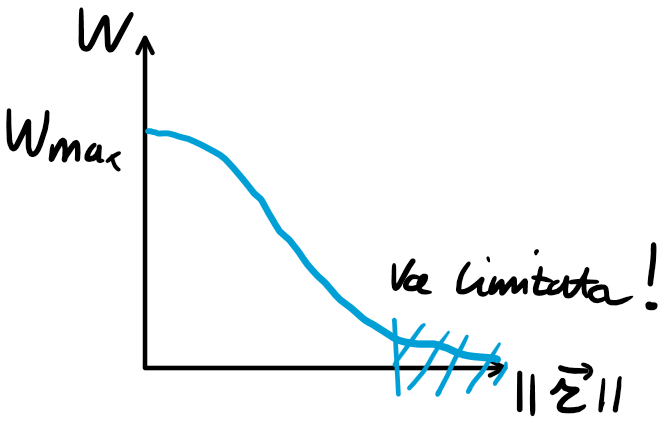
\includegraphics[width = 0.4\textwidth]{gfx/Configurazioni}}\quad
\subfloat[][\emph{}\label{def:Errori}]
{%
\begin{minipage}[b]{0.4\textwidth}
\begin{itemize}
\item $\lVert\vec{r}\rVert \rightarrow \infty$, allora $W \rightarrow 0$ ma così non è: le macromolecole hanno lunghezza finita.
\item Non è detto che le macromolecole si distribuiscano con configurazioni a campana.
\end{itemize}
\end{minipage}%
}
\caption{Errori nella formulazione della legge delle configurazioni}
\label{fig:ErroreLeggeConfigurazioni}
\end{figure}

Nonostante gli errori, basandosi su analisi statistiche si è visto che questa approssimazione è soddisfacente a livello analitico.
\begin{equation}
\begin{cases}
\left\langle \vec{r}\right\rangle &= 0 \quad\textup{La distanza di tutti i vettori è mediamente nulla}\\
\left\langle \lVert \vec{r} \rVert \right\rangle &= \frac{3}{2}\rho^2 \quad\textup{Descrive quanto òa campana sia aperta}
\end{cases}
\end{equation}
Allora tornando all'equazione di Boltzman
\begin{equation}
S = S_0 + K_b\ln\left(\frac{e^{-\frac{r^2}{\rho^2}}}{(\sqrt{\pi}\rho)^3}\right) = S_0 - K_b \frac{r^2}{\rho^2}
\end{equation}
Supponendo che $\frac{\partial S}{\partial l} \approx \frac{\partial S}{\partial r}$, infatti possiamo anche assumere che: $\Delta l \approx \lVert \vec{r} - \vec{r_0}\rVert$ per via dell'allungamento delle macromolecole per l'imposizione di una forza esterna.
\begin{equation}
\begin{split}
F &= - T\frac{\partial S}{\partial r}\Big|_{T,V}\\
&= T K_b^2 \frac{r}{\rho^2} = 2 K_b T \frac{r}{\rho^2}\\
\vec{F} &= 2 \frac{K_b T}{\rho^2}\vec{r}
\end{split}
\end{equation}

\section{Ulteriori ragionamenti}
\begin{equation}
\left\langle \vec{F} \right\rangle = 0 \Leftrightarrow \left\langle \vec{r}\right\rangle = 0
\end{equation}
Possibile che aumentando la temperatura aumenti anche la rigidezza del materiale.

Quando si tira la molecola la si sta ordinando maggiormente. Perciò più si tira il materiale più presenterà rigidezza all'aumentare della temperatura proprio ad evitare il maggiore allineamento delle macromolecole.
Di fatti è come se la rigidezza fosse direttamente proporzionale alla temperatura.

\paragraph{Forza di richiamo di origine entropica (non energetica)}
Tirando, il materiale perde di entropia per il maggiore ordine delle molecole.
Il sistema vorrebbe tornare allo stato di equilibrio e non a quello deformato.
Allora alza la temperatura per tornare ad uno stato di maggiore disordine.

\begin{equation}
\begin{cases}
\epsilon = \frac{\Delta L}{L_0}\\
\sigma = E\epsilon
\end{cases}
\end{equation}
la gomma si comporta come in figura \ref{fig:ComportamentoElastomeri}: allora sono stati sviluppati dei modelli che aderiscono a questi dati sperimentali, detti anche \textbf{Modelli ai grandi sforzi}
\begin{figure}
\centering
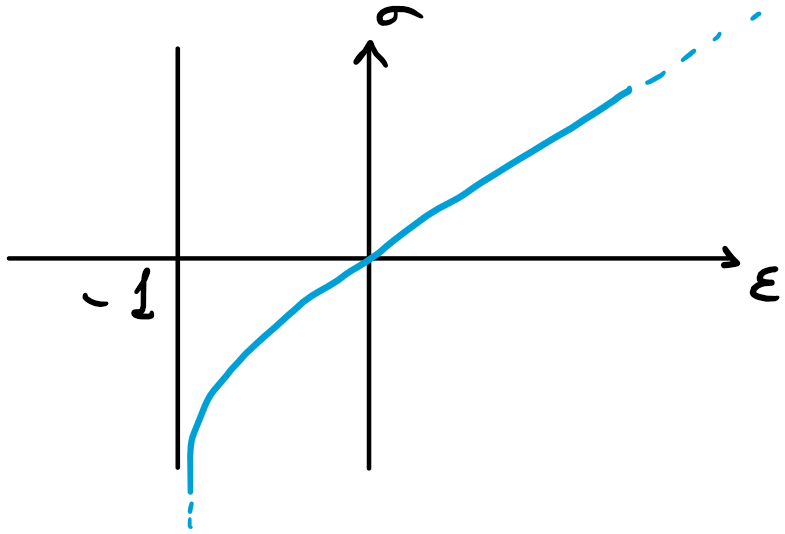
\includegraphics[width = 0.5\textwidth]{gfx/ComportamentoElastomeri}
\caption{Comportamento "singolare" degli elastomeri}
\label{fig:ComportamentoElastomeri}
\end{figure}